\documentclass[13pt,a4paper]{article}
\usepackage[spanish,es-nodecimaldot]{babel}	% Utilizar español
\usepackage[utf8]{inputenc}					% Caracteres UTF-8
\usepackage{graphicx}						% Imagenes
\usepackage[hidelinks]{hyperref}			% Poner enlaces sin marcarlos en rojo
\usepackage{fancyhdr}						% Modificar encabezados y pies de pagina
\usepackage{float}							% Insertar figuras
\usepackage[textwidth=390pt]{geometry}		% Anchura de la pagina
\usepackage[nottoc]{tocbibind}				% Referencias (no incluir num pagina indice en Indice)
\usepackage{enumitem}						% Permitir enumerate con distintos simbolos
% \usepackage[T1]{fontenc}					% Usar textsc en sections
\usepackage{amsmath}						% Símbolos matemáticos
\usepackage[ruled,vlined]{algorithm2e}      % Pseudocódigo
\usepackage{xcolor}
\usepackage{listings}
% Para que acepten tíldes los listing
\lstset{     
     literate=%
         {á}{{\'a}}1
         {é}{{\'e}}1
         {í}{{\'i}}1
         {ó}{{\'o}}1
         {ú}{{\'u}}1
         {Á}{{\'A}}1
         {É}{{\'E}}1
         {Í}{{\'I}}1
         {Ó}{{\'O}}1 
         {Ú}{{\'U}}1
         {ñ}{{\~n}}1 
         {Ñ}{{\~N}}1 
         {¿}{{?``}}1 
         {¡}{{!``}}1
}
\usepackage{dsfont}
\usepackage{caption, subcaption}

% ==============================================================================

\usepackage{caption}
\usepackage[section]{placeins}
\makeatletter
\def\fps@figure{H}
\makeatother

\usepackage{booktabs}
\usepackage{longtable}
\usepackage{array}
\usepackage{multirow}
\usepackage{wrapfig}
\usepackage{colortbl}
\usepackage{pdflscape}
\usepackage{tabu}
\usepackage{threeparttable}
\usepackage{threeparttablex}
\usepackage[normalem]{ulem}
\usepackage{makecell}
\usepackage[bottom]{footmisc}

% ==============================================================================
% ==============================================================================

% Comando para poner el nombre de la asignatura
\newcommand{\asignatura}{TSCAO}
\newcommand{\autor}{Ignacio Vellido Expósito}
\newcommand{\email}{ignaciove@correo.ugr.es}
\newcommand{\titulo}{Metaheurísticas}
\newcommand{\subtitulo}{Trabajo final}

% Configuracion de encabezados y pies de pagina
\pagestyle{fancy}
\lhead{\autor{}}
\rhead{\asignatura{}}
\lfoot{Máster Ciencia de Datos e Ingeniería de Computadores}
\cfoot{}
\rfoot{\thepage}
\renewcommand{\headrulewidth}{0.4pt}		% Linea cabeza de pagina
\renewcommand{\footrulewidth}{0.4pt}		% Linea pie de pagina

% ==============================================================================
% ==============================================================================

\begin{document}
    \pagenumbering{gobble}
    % ==============================================================================
% Pagina de titulo
\begin{titlepage}
    \begin{minipage}{\textwidth}
        \centering

        
\includegraphics[scale=0.5]{img/ugr.png}\\

        \textsc{\Large \asignatura{}\\[0.2cm]}
        \textsc{MÁSTER CIENCIA DE DATOS E INGENIERÍA DE COMPUTADORES}\\[1cm]

        \noindent\rule[-1ex]{\textwidth}{1pt}\\[1.5ex]
        \textsc{{\Huge \titulo\\[0.5ex]}}
        \textsc{{\Large \subtitulo\\}}
        \noindent\rule[-1ex]{\textwidth}{2pt}\\[2.5ex]

        \end{minipage}

        \vspace{0.3cm}

        \begin{minipage}{\textwidth}

        \centering

        \textbf{Autor}\\ {\autor{} \\ ignaciove@correo.ugr.es}\\[1.5ex]
        \vspace{0.4cm}

        
\includegraphics[scale=0.3]{img/etsiit.jpeg}
        
\includegraphics[scale=0.6]{img/master.png}

        \vspace{0.7cm}
        \textsc{Escuela Técnica Superior de Ingenierías Informática y de Telecomunicación}\\
        \vspace{1cm}
        \textsc{Curso 2020-2021}
    \end{minipage}
\end{titlepage}
% ==============================================================================
    
    \pagenumbering{arabic}    
    \newpage

    % ==============================================================================

\section{Maximum Diversity Problem (MD)}

\subsection{Búsqueda bibliográfica}

% https://www.scopus.com/results/results.uri?editSaveSearch=&sort=cp-f&src=s&nlo=&nlr=&nls=&sid=0e91577fead34b1c9e4d6e2f33578357&sot=b&sdt=sisr&cluster=scosubjabbr%2c%22COMP%22%2ct&sl=40&s=TITLE-ABS-KEY%28maximum+diversity+problem%29&ref=%28mdp%29&origin=resultslist&zone=leftSideBar&txGid=c96d17e4d26110d2035d852c0e3d93cc

\begin{itemize}
    \item Lopez-Pires, Fabio & Vera, Katherine & Baran, Benjamin & Sandoya, Fernando. (2017). Multi-Objective Maximum Diversity Problem. 10.1109/CLEI.2017.8226423.
    \item Marti, Rafael & Gallego, Micael & Duarte, Abraham. (2010). A branch and bound algorithm for the maximum diversity problem. European Journal of Operational Research. 200. 36-44. 10.1016/j.ejor.2008.12.023. 
    \item Aringhieri, Roberto & Cordone, Roberto. (2008). Tabu Search versus GRASP for the maximum diversity problem. 4OR. 6. 10.1007/s10288-007-0033-9. 
    \item Parreño, Francisco & ÁLvarez-Valdés, Ramón & Marti, Rafael. (2020). Measuring Diversity. A review and an empirical analysis. European Journal of Operational Research. 289. 10.1016/j.ejor.2020.07.053. 
    \item Marti, Rafael & Martínez-Gavara, Anna & Sánchez-Oro, Jesús. (2021). The capacitated dispersion problem: an optimization model and a memetic algorithm. Memetic Computing. 13. 10.1007/s12293-020-00318-1. 
    \item Marti, Rafael & Gallego, Micael & Duarte, Abraham & G. Pardo, Eduardo. (2013). Heuristics and metaheuristics for the maximum diversity problem. Journal of Heuristics - HEURISTICS. 19. 1-25. 10.1007/s10732-011-9172-4. 
    \item Silva, Geiza & Ochi, Luiz & Martins, Simone. (2004). Experimental Comparison of Greedy Randomized Adaptive Search Procedures for the Maximum Diversity Problem. Lecture Notes on Computer Science. 3059. 498-512. 10.1007/978-3-540-24838-5_37. 
    \item Zhou, Yangming & Hao, Jin-Kao & Duval, Beatrice. (2017). Opposition-Based Memetic Search for the Maximum Diversity Problem. IEEE Transactions on Evolutionary Computation. 21. 731-745. 10.1109/TEVC.2017.2674800. 
    \item Gallego, Micael & Duarte, Abraham & Laguna, Manuel & Marti, Rafael. (2009). Hybrid heuristics for the maximum diversity problem. Computational Optimization and Applications. 44. 411-426. 10.1007/s10589-007-9161-6. 
    \item Silva, Geiza & Andrade, Marcos & Ochi, Luiz & Martins, Simone & Plastino, Alexandre. (2007). New heuristics for the maximum diversity problem. J. Heuristics. 13. 315-336. 10.1007/s10732-007-9010-x. 
    \item Santos, L. & Ribeiro, Marcos & Plastino, Alexandre & Martins, Simone. (2005). A Hybrid GRASP with Data Mining for the Maximum Diversity Problem. Lecture Notes in Computer Science. 3636. 116-127. 10.1007/11546245_11. 
    \item Zhou, Yalan & Yin, Jian & Zhang, Yunong. (2009). Competitive Hopfield Network Combined With Estimation of Distribution for Maximum Diversity Problems. Systems, Man, and Cybernetics, Part B: Cybernetics, IEEE Transactions on. 39. 1048 - 1066. 10.1109/TSMCB.2008.2010220. 
    \item Andrade, Marcos & Andrade, Paulo & Martins, Simone & Plastino, Alexandre. (2005). GRASP with Path-Relinking for the Maximum Diversity Problem. Lecture Notes in Computer Science. 3503. 558-569. 10.1007/11427186_48. 
    \item Lozano, Manuel & Molina, Daniel & GarcI´a-MartI´nez, C.. (2011). Iterated greedy for the maximum diversity problem. European Journal of Operational Research. 214. 31-38. 10.1016/j.ejor.2011.04.018. 
\end{itemize}

\subsection{Pseudocódigos}

% La función objetivo en el problema PAR se calcula en base a la fórmula:

% \begin{equation}
%     f = \overline{C} + (infeasibility * \lambda)
% \end{equation}

% Siendo:

% \begin{equation}
%     \lambda = \frac{\max \{d_i \in D\}}{|R|} \quad tal\ que \ D = Distancias
% \end{equation}

% \begin{equation}
%     infeasibility = \sum_{i=0}^{|ML|} \mathds{1}(h_{C}(\overrightarrow{ML_{[i,1]}}) \neq (h_{C}(\overrightarrow{ML_{[i,2]}}) + \sum_{i=0}^{|CL|} \mathds{1}(h_{C}(\overrightarrow{CL_{[i,1]}}) = (h_{C}(\overrightarrow{CL_{[i,2]}})
% \end{equation}

% \begin{equation}
%     \overline{C} = \frac{1}{k} \sum_{c_{i}\in C} || \overrightarrow{x_j} - \overrightarrow{u_j} ||_{2}
% \end{equation}

% Que es calculada en pseudocódigo: \\

% \begin{algorithm}[H]
%     \SetAlgoLined
%         C $=$ Distancia media intra-cluster \;
%         $\lambda =$ Distancia máxima en el conjunto de datos / nº de restricciones  \;
%         inf $=$ Nº restricciones no cumplidas \;
%     \Return{C + ($\lambda *$ inf)}
%     \caption{Función objetivo}
% \end{algorithm}

% \vspace{\baselineskip}

% \begin{algorithm}[H]
%     \SetAlgoLined
%     \KwIn{Conjunto de datos, solucion, centroides}
%         Separar conjunto de datos según su cluster \;
%         \For{particion del conjunto de datos} {
%             Calcular distancia media de sus elementos al centroide correspondiente \;
%         }        
%     \Return{C}
%     \caption{Distancia media intra-cluster}
% \end{algorithm}

% \vspace{\baselineskip}

% \begin{algorithm}[H]
%     \SetAlgoLined
%     \SetKw{KwInFor}{in}
%     \KwIn{s: solución}
%         inf $=$ 0 \;
%         \For{r \textbf{in} $lista\_restricciones$} {
%             \uIf{r $=$ ML \textbf{and} $s[r[0]] \neq s[r[1]]$} {
%                 inf++ \;
%             }            
%             \uElseIf{r $=$ CL \textbf{and} $s[r[0]] = s[r[1]]$} {
%                     inf++ \;
%             }
%         }
%     \Return{inf}
%     \caption{Infeasibility}
% \end{algorithm}

\subsection{Operador de vecindario}

\subsection{Algoritmo de búsqueda local}

\subsection{Algoritmo genético}

% Representación (cromosomas)
% Operador mutación
% Operador cruce
% Inicialización de población

\section{Multidimensional two-way number partitioning problem (M2NP)}

\subsection{Búsqueda bibliográfica}

% https://www.scopus.com/results/results.uri?src=s&st1=&st2=&sot=b&sdt=b&origin=searchbasic&rr=&sl=59&s=TITLE-ABS-KEY(multidimensional%20two%20way%20number%20partitioning)&searchterm1=multidimensional%20two%20way%20number%20partitioning&searchTerms=&connectors=

\begin{itemize}
    \item Kojić, Jelena. (2010). Integer linear programming model for multidimensional two-way number partitioning problem. Computers & Mathematics with Applications. 60. 2302-2308. 10.1016/j.camwa.2010.08.024. 
    \item Alexandre Frias Faria, Sérgio Ricardo de Souza, Elisangela Martins de Sá, A mixed-integer linear programming model to solve the Multidimensional Multi-Way Number Partitioning Problem, Computers & Operations Research, Volume 127, 2021, 105133, ISSN 0305-0548.
    \item Santucci, Valentino & Baioletti, Marco & Di Bari, Gabriele & Milani, Alfredo. (2019). A Binary Algebraic Differential Evolution for the MultiDimensional Two-Way Number Partitioning Problem. 10.1007/978-3-030-16711-0_2. 
    \item Hacibeyoglu, Mehmet & Alaykiran, Kemal & ACILAR, A. Merve & Tongur, Vahit & Ülker, Erkan. (2018). A Comparative Analysis of Metaheuristic Approaches for Multidimensional Two-Way Number Partitioning Problem. Arabian Journal for Science and Engineering. 43. 10.1007/s13369-018-3155-9. 
    \item Jozef Kratica, Jelena Kojić, Aleksandar Savić,Two metaheuristic approaches for solving multidimensional two-way number partitioning problem,Computers & Operations Research,Volume 46,2014,Pages 59-68,ISSN 0305-0548,
    \item Pop, Petrica & Matei, Oliviu. (2013). A Genetic Algorithm Approach for the Multidimensional Two-Way Number Partitioning Problem. 7997. 81-86. 10.1007/978-3-642-44973-4_10. 
    \item Petrică C. Pop, Oliviu Matei,A memetic algorithm approach for solving the multidimensional multi-way number partitioning problem,Applied Mathematical Modelling,Volume 37, Issue 22,2013,Pages 9191-9202,ISSN 0307-904X,
    \item Vera, J. & Macías, Rodrigo & Heiser, Willem. (2009). A Latent Class Multidimensional Scaling Model for Two-Way One-Mode Continuous Rating Dissimilarity Data. Psychometrika. 74. 297-315. 10.1007/s11336-008-9104-x.
\end{itemize}

% MGS
% https://www.scopus.com/results/results.uri?cc=10&sort=r-f&src=s&nlo=&nlr=&nls=&sid=7659d39a8257beebb53de9c8729fa21d&sot=b&sdt=cl&cluster=scosubjabbr%2c%22COMP%22%2ct&sl=37&s=TITLE-ABS-KEY%28minimum+generating+set%29&ss=r-f&ps=r-f&editSaveSearch=&origin=resultslist&zone=resultslist

% A genetic algorithm for the minimum generating set problem

% The Complexity of Generating Minimum Test Sets for PLA's and Monotone Combinational Circuits

% The complexity of quasigroup isomorphism and the minimum generating set problem

% \vspace{\baselineskip}

% Un agricultor dispone de una superficie de 640m² para cultivar naranjos, perales, manzanos y
% limoneros. La cuestión es cómo debe distribuir la superficie entre los árboles para maximizar
% los beneficios teniendo la siguiente información:

% \begin{itemize}
%     \item Los naranjos necesitan un mínimo de 16m², los perales necesitan 4m², los manzanos 8m² y cada limonero necesita 12m².
%     \item El agricultor dispone de 900 horas de trabajo al año. Las demandas de los diferentes árboles son: cada naranjo 30 horas, cada peral 5 horas, cada manzano 10 horas y cada limonero 20 horas.
%     \item Debido a las restricciones, el agua disponible para el riego es de 200m³ al año. La demanda de agua (por año y árbol) es: naranjo: 2m³, peral 3m³, manzano: 1m³ y limonero 2m³.
%     \item Los beneficios (por año y árbol) son de 50, 25, 20 y 30 euros para los naranjos, perales, manzanos y limoneros respectivamente.
% \end{itemize}

% \vspace{\baselineskip}

% Se plantea el problema de la siguiente forma:
% \begin{lstlisting}[mathescape=true]
%     N = Número de naranjos
%     M = Número de manzanos
%     L = Número de limoneros
%     P = Número de perales

%     max    50N + 25P + 20M + 30L 
%     s.t.   16N +  4P +  8M + 12L $\leq$ 640
%            30N +  5P + 10M + 20L $\leq$ 900
%             2N +  3P +   M +  2L $\leq$ 200
%              N,    P,    M,    L $\geq$   0
% \end{lstlisting}

% \begin{figure}[t]\center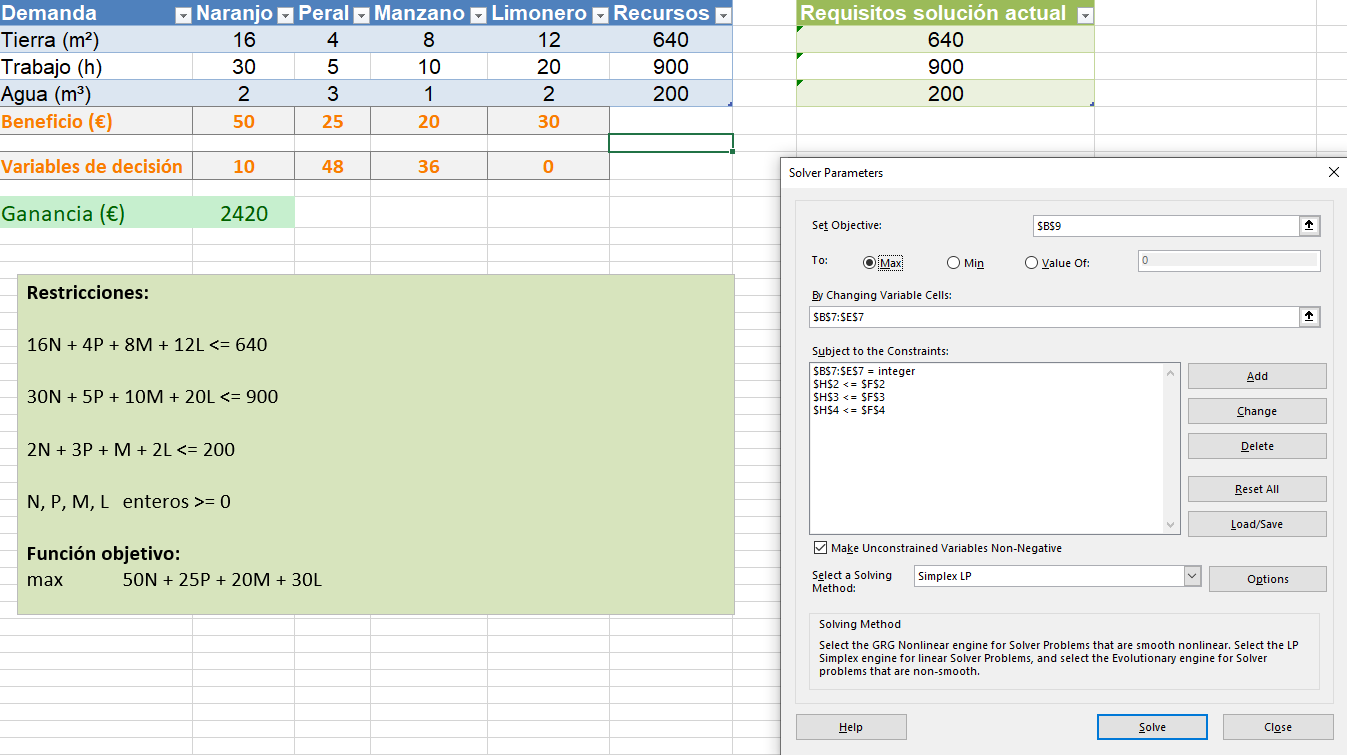
\includegraphics[width=.95\linewidth]{img/solver.png}\caption{Resolución del problema de los árboles frutales.}\end{figure}

% \begin{figure}[b]\center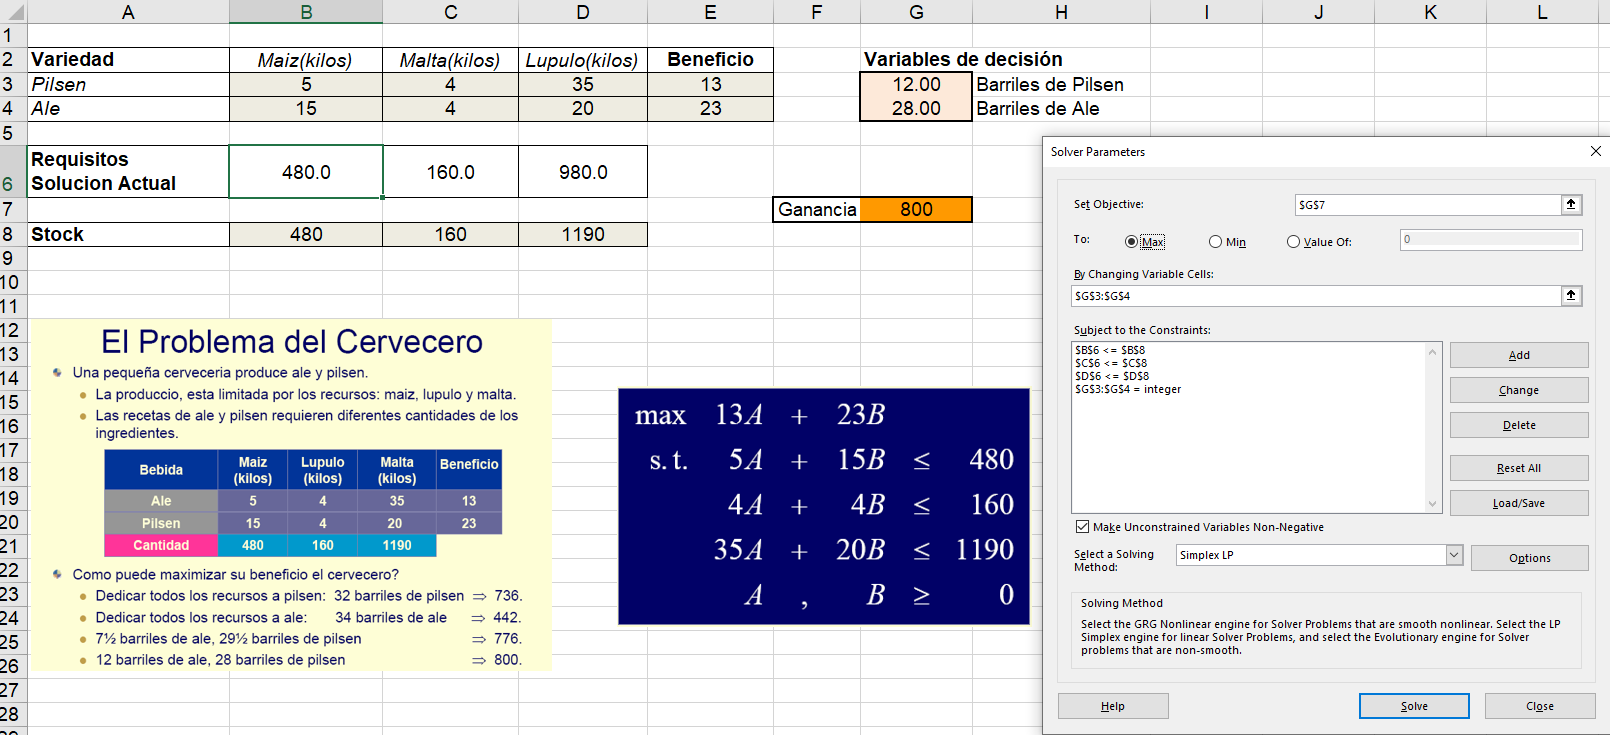
\includegraphics[width=.95\linewidth]{img/solver2.png}\caption{Resolución del problema de la cervecería.}\end{figure}

% \begin{figure}[t]\center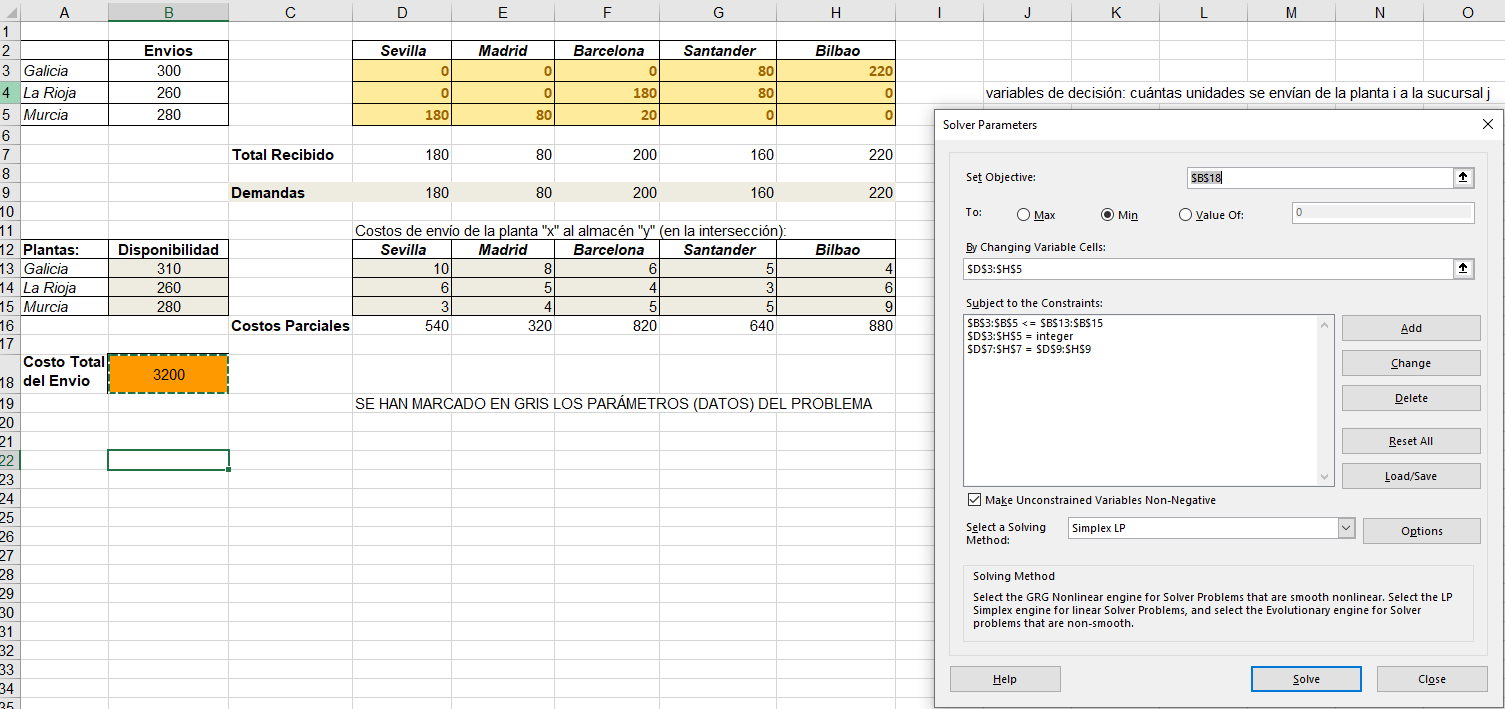
\includegraphics[width=.95\linewidth]{img/solver3.png}\caption{Resolución del problema de la distribución de mercancías.}\end{figure}

% \newpage

% \section{Parte 2}

% \begin{figure}[H]
%     \centering
%     \resizebox{0.75\columnwidth}{!}{%
%     \begin{tabular}{| l || c | c | c |} 
%         \hline
%         \textbf{Heurística} & \multicolumn{3}{c |}{\textbf{Problema}} \\
%         \Xhline{2\arrayrulewidth}
%         & bcl380 & icw1483 & bck2217 \\
%         \hline
%         Greedy & 1862 & 5032 & 7851 \\
%         \hline
%         Borukva & 1915 & 5166 & 7861 \\
%         \hline
%         Quick Borukva & 1872 & 5379 & 8117 \\
%         \hline
%         Nearest Neighbour & 2057 & 5681 & 8740 \\
%         \hline
%         Lin Kernighan Default (+ Greedy) & 1644 & 4487 & 6848 \\
%         \hline
%         Lin Kernighan 10 kicks & 1668 & 4738 & 7196 \\
%         \hline
%         Lin Kernighan 100 kicks & 1634 & 4601 & 7098 \\
%         \hline
%         Lin Kernighan + Quick Borukva & 1630 & 4501 & 6910 \\
%         \hline
%         Random & 26086 & 149247 & 297518 \\
%         \hline
%     \end{tabular}
%     }
%     \caption{Resultados de distancia de cada heurística para los diferentes problemas TSP.}
% \end{figure}

% Lin Kernighan obtiene los mejores resultados para cada uno de los problemas, a costa de un mayor tiempo de cómputo. Entre el resto (y a excepción de Nearest Neighbour) no existen diferencias suficientemente significas en la calidad de las soluciones encontradas, aunque la heurística Greedy es la que obtiene mejores resultados en estas instancias de TSP.

% \vspace{\baselineskip}

% Los cambios en los parámetros de la heurística Lin Kernighan dan resultados inconsistentes, pero apreciamos que el decremento del número de ``kicks'' (por defecto igual al número de nodos) influye negativamente en la longitud de los caminos encontrados.

% También notamos que el cambio del algoritmo inicial afecta en tiempo de cómputo pero apenas en los resultados obtenidos, siendo en general ligeramente inferiores pasando de Greedy a Quick Borukva.

% \begin{figure}[b]
%     \centering 
%     \begin{subfigure}[t]{0.3\textwidth}
%       \centering
%       \includegraphics[width=\textwidth]{img/1/G.png}
%       \caption{Greedy.}
%     \end{subfigure}
%     % \vspace{7mm}
%     % \hfill
%     \begin{subfigure}[t]{0.3\textwidth}
%         \centering
%         \includegraphics[width=\textwidth]{img/1/B.png}
%         \caption{Borukva.}
%     \end{subfigure}
%     % \hfill
%     \begin{subfigure}[t]{0.3\textwidth}
%       \centering
%       \includegraphics[width=\textwidth]{img/1/Q.png}
%       \caption{Quick Borukva.}
%     \end{subfigure}

%     % \hfill
%     \begin{subfigure}[t]{0.3\textwidth}
%         \centering
%         \includegraphics[width=\textwidth]{img/1/N.png}
%         \caption{Nearest Neighbour.}
%     \end{subfigure}
%     % \hfill
%     \begin{subfigure}[t]{0.3\textwidth}
%         \centering
%         \includegraphics[width=\textwidth]{img/1/L1.png}
%         \caption{Lin Kernighan Default.}
%     \end{subfigure}
%     % \hfill
%     \begin{subfigure}[t]{0.3\textwidth}
%         \centering
%         \includegraphics[width=\textwidth]{img/1/L10.png}
%         \caption{Lin Kernighan 10 kicks.}
%     \end{subfigure}

%     % \hfill
%     \begin{subfigure}[t]{0.3\textwidth}
%         \centering
%         \includegraphics[width=\textwidth]{img/1/L100.png}
%         \caption{Lin Kernighan 100 kicks.}
%     \end{subfigure}
%     % \hfill
%     \begin{subfigure}[t]{0.3\textwidth}
%         \centering
%         \includegraphics[width=\textwidth]{img/1/L+Q.png}
%         \caption{L.K + Quick Borukva.}
%     \end{subfigure}
%     % \hfill
%     \begin{subfigure}[t]{0.3\textwidth}
%         \centering
%         \includegraphics[width=\textwidth]{img/1/R.png}
%         \caption{Random.}
%     \end{subfigure}
%     \caption{Rutas calculadas por cada heurística para el problema bcl380.}
% \end{figure}
  
% \begin{figure}[t]
%     \centering 
%     \begin{subfigure}[t]{0.3\textwidth}
%       \centering
%       \includegraphics[width=\textwidth]{img/2/G.png}
%       \caption{Greedy.}
%     \end{subfigure}
%     % \vspace{7mm}
%     % \hfill
%     \begin{subfigure}[t]{0.3\textwidth}
%         \centering
%         \includegraphics[width=\textwidth]{img/2/B.png}
%         \caption{Borukva.}
%     \end{subfigure}
%     % \hfill
%     \begin{subfigure}[t]{0.3\textwidth}
%       \centering
%       \includegraphics[width=\textwidth]{img/2/Q.png}
%       \caption{Quick Borukva.}
%     \end{subfigure}

%     % \hfill
%     \begin{subfigure}[t]{0.3\textwidth}
%         \centering
%         \includegraphics[width=\textwidth]{img/2/N.png}
%         \caption{Nearest Neighbour.}
%     \end{subfigure}
%     % \hfill
%     \begin{subfigure}[t]{0.3\textwidth}
%         \centering
%         \includegraphics[width=\textwidth]{img/2/L1.png}
%         \caption{Lin Kernighan Default.}
%     \end{subfigure}
%     % \hfill
%     \begin{subfigure}[t]{0.3\textwidth}
%         \centering
%         \includegraphics[width=\textwidth]{img/2/L10.png}
%         \caption{Lin Kernighan 10 kicks.}
%     \end{subfigure}

%     % \hfill
%     \begin{subfigure}[t]{0.3\textwidth}
%         \centering
%         \includegraphics[width=\textwidth]{img/2/L100.png}
%         \caption{Lin Kernighan 100 kicks.}
%     \end{subfigure}
%     % \hfill
%     \begin{subfigure}[t]{0.3\textwidth}
%         \centering
%         \includegraphics[width=\textwidth]{img/2/L+Q.png}
%         \caption{L.K + Quick Borukva.}
%     \end{subfigure}
%     % \hfill
%     \begin{subfigure}[t]{0.3\textwidth}
%         \centering
%         \includegraphics[width=\textwidth]{img/2/R.png}
%         \caption{Random.}
%     \end{subfigure}
%     \caption{Rutas calculadas por cada heurística para el problema icw1483.}
% \end{figure}


% \begin{figure}[b]
%     \centering 
%     \begin{subfigure}[t]{0.3\textwidth}
%       \centering
%       \includegraphics[width=\textwidth]{img/3/G.png}
%       \caption{Greedy.}
%     \end{subfigure}
%     % \vspace{7mm}
%     % \hfill
%     \begin{subfigure}[t]{0.3\textwidth}
%         \centering
%         \includegraphics[width=\textwidth]{img/3/B.png}
%         \caption{Borukva.}
%     \end{subfigure}
%     % \hfill
%     \begin{subfigure}[t]{0.3\textwidth}
%       \centering
%       \includegraphics[width=\textwidth]{img/3/Q.png}
%       \caption{Quick Borukva.}
%     \end{subfigure}

%     % \hfill
%     \begin{subfigure}[t]{0.3\textwidth}
%         \centering
%         \includegraphics[width=\textwidth]{img/3/N.png}
%         \caption{Nearest Neighbour.}
%     \end{subfigure}
%     % \hfill
%     \begin{subfigure}[t]{0.3\textwidth}
%         \centering
%         \includegraphics[width=\textwidth]{img/3/L1.png}
%         \caption{Lin Kernighan Default.}
%     \end{subfigure}
%     % \hfill
%     \begin{subfigure}[t]{0.3\textwidth}
%         \centering
%         \includegraphics[width=\textwidth]{img/3/L10.png}
%         \caption{Lin Kernighan 10 kicks.}
%     \end{subfigure}

%     % \hfill
%     \begin{subfigure}[t]{0.3\textwidth}
%         \centering
%         \includegraphics[width=\textwidth]{img/3/L100.png}
%         \caption{Lin Kernighan 100 kicks.}
%     \end{subfigure}
%     % \hfill
%     \begin{subfigure}[t]{0.3\textwidth}
%         \centering
%         \includegraphics[width=\textwidth]{img/3/L+Q.png}
%         \caption{L.K + Quick Borukva.}
%     \end{subfigure}
%     % \hfill
%     \begin{subfigure}[t]{0.3\textwidth}
%         \centering
%         \includegraphics[width=\textwidth]{img/3/R.png}
%         \caption{Random.}
%     \end{subfigure}
%     \caption{Rutas calculadas por cada heurística para el problema bck2217.}
% \end{figure}

    % ==============================================================================
    \setlength{\parskip}{1em}
    \newpage
\end{document}

% ==============================================================================
% ==============================================================================